\documentclass[12pt, a4paper]{book}

\usepackage[english]{babel}
\usepackage[T1]{fontenc}
\usepackage[utf8]{inputenc}
\usepackage{lmodern}
\usepackage{listings}
\usepackage{tikz}
\usepackage{amsmath}
\usepackage{amssymb}
\usepackage{framed}
\usepackage{graphicx}
\usepackage{booktabs}
\usepackage{csquotes}
\usepackage{hyperref}
\usepackage[inference]{semantic}

\graphicspath{{img/}}

\usetikzlibrary{arrows, chains, decorations}

\lstset{
    language=Java,
    basicstyle=\footnotesize,
    frame=single,
    morekeywords={if,else,do,while},
    numbers=left,
    numberstyle=\tiny\color{gray},
    captionpos=below,
}

\author{Florian Thuin}
\title{LSINF2224 --- Programming methods}

\begin{document}
    \maketitle
    \tableofcontents
%%%%%%%%%%%%%%%%%%%%%%%%%%%%%%%%%%%%%%%%%%%%%%%%%%%%%%%%%%%%%%%%%%%%%%%%%%%%%%%%
% SECTION : Organization
%%%%%%%%%%%%%%%%%%%%%%%%%%%%%%%%%%%%%%%%%%%%%%%%%%%%%%%%%%%%%%%%%%%%%%%%%%%%%%%%
  \section{Organization}
  \label{sec:Organization}

  \subsection{Objectives}
  \label{sub:Objectives}
  \subsection{Synopsis}
  \label{sub:Synopsis}
  \subsection{Website}
  \label{sub:Website}
  \subsection{Course Outline}
  \label{sub:Course Outline}
  \subsection{Course material}
  \label{sub:Course material}
  \subsection{Bibliography}
  \label{sub:Bibliography}
  \subsection{Labs}
  \label{sub:Labs}
  \subsubsection{Goals}
  \label{subs:Goals}
  \subsubsection{Implementation}
  \label{subs:Implementation}
  \subsubsection{Languages}
  \label{subs:Languages}
  \subsubsection{Software}
  \label{subs:Software}
  \subsubsection{Assignments}
  \label{subs:Assignments}
  \subsection{Evaluation}
  \label{sub:Evaluation}


%%%%%%%%%%%%%%%%%%%%%%%%%%%%%%%%%%%%%%%%%%%%%%%%%%%%%%%%%%%%%%%%%%%%%%%%%%%%%%%%
% SECTION : Demonstration
%%%%%%%%%%%%%%%%%%%%%%%%%%%%%%%%%%%%%%%%%%%%%%%%%%%%%%%%%%%%%%%%%%%%%%%%%%%%%%%%
  \section{Demonstration}
  \label{sec:Demonstration}

  The goal of this initial demo is to show how we can automatically verify a
  Java program. We will use \textit{ESC/Java} that uses \textbf{enriched formal
  specifications} to make automated checks.

  \subsection{Binary Search: Implementation}
  \label{sub:Binary Search: Implementation}

  \lstinputlisting[language=Java, caption={Implementation of a binary search in
  Java}]{BinarySearch.java}

  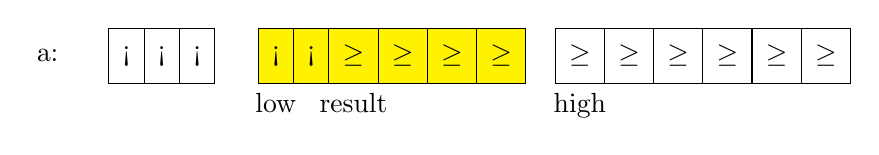
\begin{tikzpicture}
      \tikzstyle{element}=[rectangle, draw, inner sep=5pt, outer sep=0pt, minimum height=0.7cm]
      \draw (0,0) node(a) {a:};
      \node[element, right of=a] (b) {<};
      \node[element, right=0cm of b] (c) {<};
      \node[element, right=0cm of c] (d) {<};
      \node[element, right of=d, fill=yellow] (f) {<};
      \node[below=0cm of f] (low) {low};
      \node[element, right=0cm of f, fill=yellow] (g) {<};
      \node[element, right=0cm of g, fill=yellow] (h) {$\ge$};
      \node[below=0cm of h] (result) {result};
      \node[element, right=0cm of h, fill=yellow] (i) {$\ge$};
      \node[element, right=0cm of i, fill=yellow] (j) {$\ge$};
      \node[element, right=0cm of j, fill=yellow] (k) {$\ge$};
      \node[element, right of=k] (l) {$\ge$};
      \node[below=0cm of l] (high) {high};
      \node[element, right=0cm of l] (m) {$\ge$};
      \node[element, right=0cm of m] (n) {$\ge$};
      \node[element, right=0cm of n] (o) {$\ge$};
      \node[element, right=0cm of o] (p) {$\ge$};
      \node[element, right=0cm of p] (q) {$\ge$};
  \end{tikzpicture}

%%%%%%%%%%%%%%%%%%%%%%%%%%%%%%%%%%%%%%%%%%%%%%%%%%%%%%%%%%%%%%%%%%%%%%%%%%%%%%%%
%%%%%%%%%%%%%%%%%%%%%%%%%%%%%%%%%%%%%%%%%%%%%%%%%%%%%%%%%%%%%%%%%%%%%%%%%%%%%%%%
% CHAPTER : Foundations
%%%%%%%%%%%%%%%%%%%%%%%%%%%%%%%%%%%%%%%%%%%%%%%%%%%%%%%%%%%%%%%%%%%%%%%%%%%%%%%%
%%%%%%%%%%%%%%%%%%%%%%%%%%%%%%%%%%%%%%%%%%%%%%%%%%%%%%%%%%%%%%%%%%%%%%%%%%%%%%%%
  \chapter{Foundations}
  \label{chap:Foundations}

%%%%%%%%%%%%%%%%%%%%%%%%%%%%%%%%%%%%%%%%%%%%%%%%%%%%%%%%%%%%%%%%%%%%%%%%%%%%%%%%
% SECTION : Introduction
%%%%%%%%%%%%%%%%%%%%%%%%%%%%%%%%%%%%%%%%%%%%%%%%%%%%%%%%%%%%%%%%%%%%%%%%%%%%%%%%
  \section{Introduction}
  \label{sec:Introduction}

In this chapter, we will discuss the foundations of proofs, what can be done
and what cannot, why and how. \newline

The basis of this course are the programs. Every program has a language, the
language we will use is a mix between Java and Pascal (it should be very
easy for you to read it) that has a minimal set of interesting constructs
because we only need assignment, sequence, choice (conditions) and loops.
\newline

\paragraph{Example} computing $a^b$
\begin{lstlisting}[numbers=left,caption={Example of code},label=code:basiccode]
{
    x=b;
    y=1;
    while (x>0) do {
        y=y*a;
        x=x-1;
    }
}
\end{lstlisting}

Each language has a syntax (the structure of program text), a static semantics
(typing, identifier scopes) that defines well-formed programs and a dynamic
semantics that defines the program behaviour (including runtime errors).
\newline

\begin{verbatim}
stmt  ::= var=expr;
       |  {stmts}
       |  if (bexpr) then stmt else stmt
       |  while (bexpr) do stmt
stmts ::= stmt*
\end{verbatim}

In this paper, we will only discuss well-formed programs without typing, and we
don't care about static semantics: no variable declaration, no types here.
\newline

In this chapter, the goal is to talk about what is program, what is a property
and how we can build a proof system to automate the proof of properties on
programs.

  \begin{figure}[!ht]
      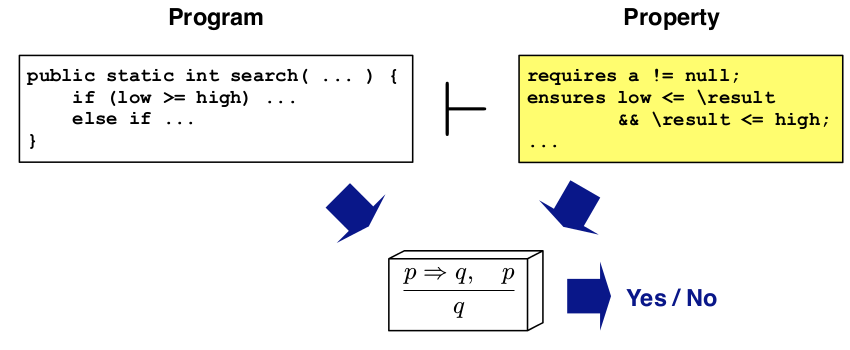
\includegraphics[width=\linewidth]{program_proofs.png}
      \caption{Program proofs}
  \end{figure}
%%%%%%%%%%%%%%%%%%%%%%%%%%%%%%%%%%%%%%%%%%%%%%%%%%%%%%%%%%%%%%%%%%%%%%%%%%%%%%%%
 % SECTION : Foundations
%%%%%%%%%%%%%%%%%%%%%%%%%%%%%%%%%%%%%%%%%%%%%%%%%%%%%%%%%%%%%%%%%%%%%%%%%%%%%%%%
  \section{Foundations}
  \label{sec:Foundations}

\subsection{Expressions}
\label{sub:Expressions}


Programs are made of \textit{expressions} that are each part that computes a
value. The syntax for expression is the following:

\begin{verbatim}
expr  ::= nexpr|bexpr|...
nexpr ::= number|var|-nexpr|nexpr+nexpr|...
bexpr ::= true|false|!bexpr|bexpr&&bexpr|...
\end{verbatim}

Expressions are weither \textit{numerical expression} $nexpr \subset expr$
($2,x, abs(y), a+b$) or boolean expressions $bexpr \subset expr$
($a[k]>0, x==2, empty(l)$). We will assume that each expression is well-typed
and pure (without side effect\footnote{Side effects are modifications of global
variables or static variables or interaction with the world that may lead to
variation between executions}). \newline

\subsection{Execution state}
\label{sub:Execution state}

\begin{figure}[!ht]
    \centering
    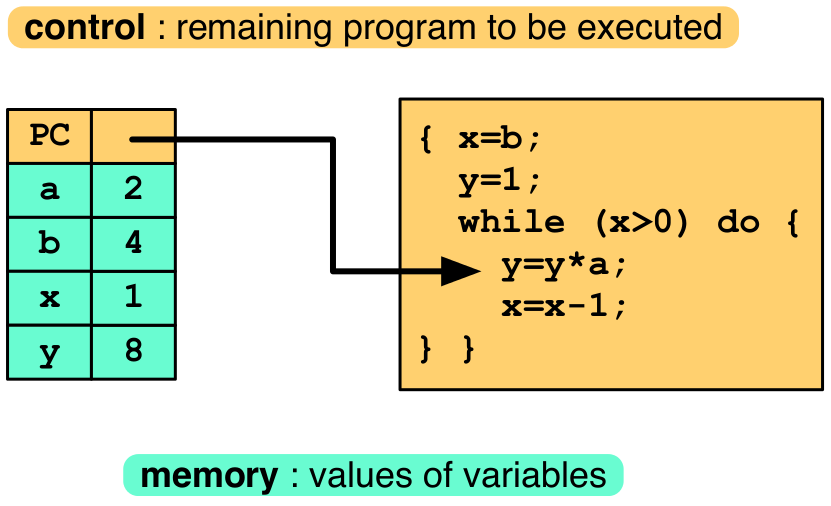
\includegraphics[width=0.6\linewidth]{execution_state.png}
    \caption{Execution state}
\end{figure}

\paragraph{How do we store states?} We know the value of the variables (the
result of evaluating expressions as integer or boolean in our examples). The
set of data values $D$ for each state contains all the boolean
$b \in B = {true, false}$, such that $B \subset D$. \newline

Those data values $d \in D$ are stored in \textit{stores} (memory) that are
functions that maps variables to their values. $\sigma$ is a store, $\Sigma$ is
the set of all the functions from the variables to their domains, $var$ is a
variable such that $\sigma \in \Sigma = var \rightarrow D$ with $\sigma(V)$ the
value of $V$ in $\sigma$.

\begin{minipage}{\linewidth}
    \begin{minipage}{0.4\linewidth}
        $$\sigma(a) = 2$$
        $$\sigma(y)=8$$
    \end{minipage}
    \begin{minipage}{0.4\linewidth}
        \centering
        \begin{tabular}{ll}
            \toprule
            a & 2 \\
            \midrule
            b & 4 \\
            \midrule
            x & 1 \\
            \midrule
            y & 8 \\
            \bottomrule
        \end{tabular}
    \end{minipage}
\end{minipage}
\bigskip

We can update the stores by modifying the value of the variables that we
write $\sigma[V := d] = \sigma'$ such that

\begin{itemize}
    \item $\sigma'(V') = d$ when $V' =V$
    \item $\sigma'(V') = \sigma(V')$ otherwise.
\end{itemize}

\begin{minipage}{\linewidth}
    \begin{minipage}{0.4\linewidth}
        $$\sigma[y := 16]$$
    \end{minipage}
    \begin{minipage}{0.4\linewidth}
        \centering
        \begin{tabular}{ll}
            \toprule
            a & 2 \\
            \midrule
            b & 4 \\
            \midrule
            x & 1 \\
            \midrule
            y & \textcolor{red}{16} \\
            \bottomrule
        \end{tabular}
    \end{minipage}
\end{minipage}

A \textbf{control state} is the program (or the residual program) to be executed
denoted $S \in stmt$. A \textbf{global state} is a \textit{configuration}, i.e.
an abstract machine about to execute a program $S$ from a store $\sigma$,
denoted $(S,\sigma) \in stmt \times \Sigma$ (or control $\times$ store).

\begin{figure}[!ht]
    \centering
    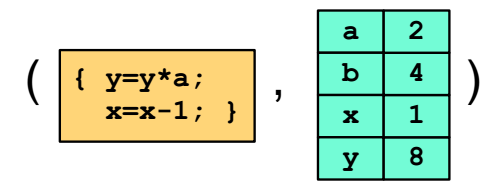
\includegraphics[width=0.5\linewidth]{global_state.png}
    \caption{Representation of a global state}
\end{figure}

\subsection{Semantics}
\label{sub:Semantics}

In this part, we will describe the semantics used for expressions and boolean
expressions. \newline

As we consider expression in programs (only \textit{pure}\footnote{that does
not have a side-effect} expression where $\sigma$ does not change), we have to
extend $\sigma : V \rightarrow D$ to a valuation on $expr$:

$$
\sigma : expr \rightarrow D
$$

\begin{eqnarray}
    \textcolor{red}{\sigma(}\textcolor{green!60!black}{42}\textcolor{red}{)} & = & \textcolor{red}{42} \\
    \textcolor{red}{\sigma(}\textcolor{green!60!black}{true}\textcolor{red}{)} & = & \textcolor{red}{true} \\
    \textcolor{red}{\sigma(}\textcolor{green!60!black}{E1*E2}\textcolor{red}{)} & = & \textcolor{red}{\sigma(}\textcolor{green!60!black}{E1}\textcolor{red}{) \times \sigma(}\textcolor{green!60!black}{E2}\textcolor{red}{)} \\
    \textcolor{red}{\sigma(}\textcolor{green!60!black}{E1<=E2}\textcolor{red}{)} & = & \textcolor{red}{\sigma(}\textcolor{green!60!black}{E1}\textcolor{red}{) \le \sigma(}\textcolor{green!60!black}{E2}\textcolor{red}{)}
\end{eqnarray}

The parts in \textcolor{green!60!black}{green} are syntax, the parts in
\textcolor{red}{red} are semantics. \newline

For a boolean expression $B \in bexpr$, we define semantics as follow:

\begin{itemize}
    \item $[[B]] = \{\sigma \mid \sigma(B)\}$ is the set of stores in which $B$
    is true.
    \item $[[\lnot B]] = \{\sigma \mid \lnot \sigma(B)\}$ is the set of stores
    in which $B$ is false.
\end{itemize}

For example,
$$
\textcolor{red}{[[}\textcolor{green!60!black}{E1<=E2}\textcolor{red}{]] = \{\sigma \mid \sigma(}\textcolor{green!60!black}{E1}\textcolor{red}{) \le \sigma(}\textcolor{green!60!black}{E2}\textcolor{red}{)\}}
$$

\subsection{Transition}
\label{sub:Transition}

We define a \textbf{transition relation} $\longrightarrow$ between
configurations :

$$(S,\sigma) \longrightarrow (S',\sigma')$$

means:

\begin{itemize}
    \item executions of one step of $S$ from $\sigma$ yields $\sigma'$
    \item $S'$ being the remainder of $S$ after that step
\end{itemize}

The transition relation $\longrightarrow$ defines an \textbf{operational
semantics} for programs. The operational semantics will help us to know the
meaning of the instructions step-by-step and thus to get from \textit{pre} to
\textit{post}.

\begin{figure}[!ht]
    \centering
    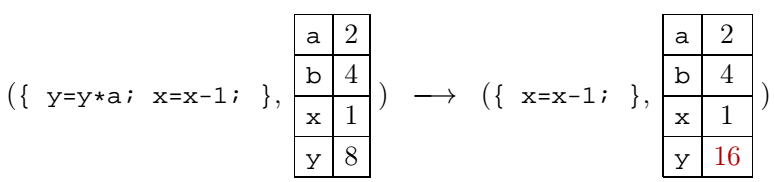
\includegraphics[width=0.8\linewidth]{transition1.png}
    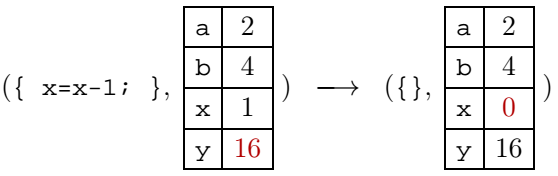
\includegraphics[width=0.6\linewidth]{transition2.png}
    \caption{Transitions: Example}
\end{figure}

The transition relation is defined by \textit{induction} on program structure as
\textbf{inference rules}. \newline

\paragraph{Example} The instruction block $\{S_1 S_2 \ldots S_n\}$

\begin{itemize}
    \item IF $(S_1, \sigma) \longrightarrow (S_{1}^{'},\sigma')$ THEN
    $(\{S_1S_2\ldots S_n\}, \sigma) \longrightarrow (\{S_1^{'}S_2\ldots S_n\},\sigma')$
    \item IF $S_1 = \{\}$ (i.e. $S_1$ is done) THEN $(\{S_1S_2\ldots S_n\},\sigma) \longrightarrow (\{S_2\ldots S_n\}, \sigma)$
\end{itemize}

This is a \textbf{structural operational semantics} (SOS).

\subsection{Inference}
\label{sub:Inference}

Now that we have the semantics with us, we will need rules to decide the value
of the next state. We denote an inference rule as:

$$\frac{\phi_{1} \ldots \phi_{n}}{\phi}$$

which means that

\begin{itemize}
    \item if $\phi_1$ and \ldots and $\phi_n$ then $\phi$
    \item from $\phi_1$ and \ldots and $\phi_n$ we can deduce $\phi$
\end{itemize}

Example:

$$
\frac{(S,\sigma) \longrightarrow (S', \sigma')}
{(\{S\ SS\},\sigma) \longrightarrow (\{S'\ SS\}, \sigma')}
$$

Axioms are particular cases of rules, because they are \textit{true} without
condition. We denote them as:

$$
\frac{}
{\ \phi \ }
$$

which means

\begin{itemize}
    \item $\phi$ is true
    \item $\phi$ is an axiom
\end{itemize}

Example:
$$
\frac{}
{(\{ \{ \} \ SS, \sigma \}) \longrightarrow (\{ SS \}, \sigma)}
$$
means that the \textit{empty program} followed by a sequence of instructions can
be reduced to this sequence of instructions. \newline

An \textbf{inference system} is a set of inference rules $R$ including axioms.
Axioms and inference rules can be derivated to discover new rules that will lead
to the searched proof. \newline

A \textbf{derivation} of $\phi$ in $R$ (denoted $\vdash_R \phi$) is a sequence
of formulae $\phi_0,\phi_1,\ldots,\phi_n$ ending with $\phi_n \equiv \phi$ such
that each formula $\phi_k$ results from applying a rule of $R$ to preceding
formulae $\phi_l$ with $l<k$. \newline

We can formalize the construction by derivation from $R^0$ (the set of axioms):

\begin{eqnarray}
R^{0}   & = & \{\phi \mid \frac{}{\ \phi \ } \exists R\} \\
R^{k+1} & = & R^{k} \cup \{ \phi \mid \frac{\phi_{1} \ldots \phi_{n}}{\phi}
\in R \land \phi_{1}\ldots\phi_{n} \in R^{k} \} \\
R^{*}   & = & \bigcup_{k} R^{k}
\end{eqnarray}

$$
\vdash_{R} \phi \iff \phi \in R^{*}
$$

\subsection{Transition rules as inference rules}
\label{sub:Transition rules as inference rules}

In this part, we will write down transition rules as inference rules. We will
do it for each element of our language: assignment, sequence, condition
(choice), loop.

\paragraph{Assignment V=E;}

$$
\frac{}
{(V=E;,\sigma) \longrightarrow (\{ \}, \sigma [V := \sigma (E)] )}
$$

\paragraph{Sequence \{S SS\}} (S in the instruction, SS is the residual program
to be executed)

$$
\frac{(S,\sigma) \longrightarrow (S',\sigma')}
{(\{ S\ SS \} , \sigma ) \longrightarrow (\{S'\ SS\}, \sigma')}
$$

$$
\frac{}
{(\{ \{ \} SS\}, \sigma) \longrightarrow (\{ SS \}, \sigma)}
$$

\noindent \textbf{Condition} \verb#if# $(B)$ \verb#then# $S_{1}$ \verb#else# $S_{2}$

$$
\frac{}
{(\textrm{if } (B) \textrm{ then } S_{1} \textrm{ else } S_{2}, \sigma) \longrightarrow (S_{1}, \sigma)}
\ \sigma(B)
$$

$$
\frac{}
{(\textrm{if } (B) \textrm{ then } S_{1} \textrm{ else } S_{2}, \sigma) \longrightarrow (S_{2}, \sigma)}
\ \lnot\sigma(B)
$$

\noindent \textbf{Loop} \verb#while# (B) \verb#do# S

$$
\frac{}
{(\textrm{while } (B) \textrm{ do } S, \sigma) \longrightarrow (\{ S \textrm{ while } (B) \textrm{ do } S\}, \sigma)}
\sigma(B)
$$

$$
\frac{}
{(\textrm{while } (B) \textrm{ do } S, \sigma) \longrightarrow (\{ \}, \sigma)}
\lnot\sigma(B)
$$

\subsection{Runs, Termination, Divergence}

A program terminates iff the execution leads to the empty program (an empty
sequence of instructions). \newline

$(S_{0}, \sigma_{0}) \longrightarrow^{*} (S_{k}, \sigma_{k})$ iff there is a
\underline{finite} sequence

$$
(S_{0}, \sigma_{0}) \longrightarrow (S_{1}, \sigma_{1}) \longrightarrow \ldots
\longrightarrow (S_{k}, \sigma_{k})
$$

$(S, \sigma)$ \textit{terminates} in
$\sigma'$ iff $(S, \sigma) \longrightarrow^{*} (\{\}, \sigma')$ (with
$\longrightarrow^{*}$ meaning a finite number of steps)

$(S_{0}, \sigma_{0}) \longrightarrow^{\omega}$ iff there is an
\underline{infinite} sequence ($\omega$ means infinite enumerable)

$$
(S_{0}, \sigma_{0}) \longrightarrow (S_{1}, \sigma_{1}) \longrightarrow \ldots
$$

$(S,\sigma)$ \textit{diverges} iff $(S,\sigma) \longrightarrow^{\omega}$

\paragraph{Semantics: Partial Correctness}

We define the semantics of a program $S$ as a function $[[S]]: \sum \rightarrow 2^{\Sigma}$ \newline

initial store $\rightarrow$ final store \newline

Partial correctness semantics:
$$
[[S]](\sigma) = \{\sigma' \mid (S,\sigma) \longrightarrow^{*} (\{\}, \sigma')\}
$$
where $[[S]](\sigma)$ is the set of possible final stores after executing $S$
from $\sigma$

\paragraph{Semantics (Set-Based Version)}

For convenience, it is useful to define $[[S]]$ on sets of initial states. \newline

For a set of stores $X \subseteq \Sigma$,
$$
[[S]](X) = \bigcup_{\sigma \in X} [[S]](\sigma)
$$

\begin{center}
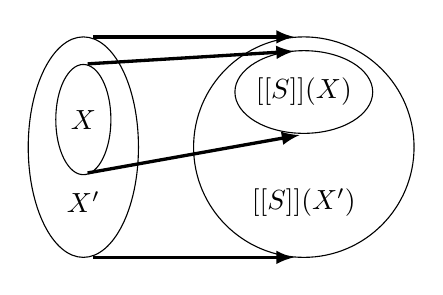
\begin{tikzpicture}[scale=0.7]
  \tikzstyle{suite}=[->,>=stealth’,thick,rounded corners=4pt]

  \draw (1,1) ellipse (1 and 2); % Right big ellipse
  \draw (1,1.5) ellipse (0.5 and 1); % Right little ellipse
  \node (A) at (1, 1.5) {$X$};
  \node (B) at (1, 0.0) {$X'$};
  \draw (5, 1) circle (2); % Right circle
  \draw (5, 2) ellipse (1.25 and 0.75); % Right ellipse in circle
  \node (C) at (5, 2) {$[[S]](X)$};
  \node (D) at (5, 0) {$[[S]](X')$};
  \node (E) at (1, 3) {}; % Top-left node
  \node (F) at (5, 3) {}; % Top-right node
  \draw[->,>=latex, very thick] (E)--(F); % Top arrow
  \node (G) at (1,-1) {};
  \node (H) at (5,-1) {};
  \draw[->,>=latex, very thick] (G)--(H); % Bottom arrow
  \node (I) at (0.9, 2.5) {};
  \node (J) at (5, 2.75) {};
  \draw[->,>=latex, very thick] (I)--(J); % Top-ellipse arrow
  \node (K) at (0.9, 0.5) {};
  \node (L) at (5.1, 1.25) {};
  \draw[->,>=latex, very thick] (K)--(L); % Bottom-ellipse arrow
\end{tikzpicture}
\end{center}

\paragraph{Property}: [[S]] is monotonic:

$$
X \subseteq X' \Rightarrow [[S]](X) \subseteq [[S]](X')
$$

\noindent Proof: obvious from definition \newline

Important for convergence of iterative computations \newline

\paragraph{Semantics: Total Correctness}

Distinguished value $\perp$ (bottom) denotes absence of final state (i.e.
the final state of a non-terminating program).

\textbf{Total Correctness Semantics:}
$$
{[[S]]}_{\perp}(\sigma) = [[S]](\sigma) \cup \{\perp \mid (S,\sigma) \longrightarrow^{\omega}\}
$$

${[[S]]}_{\perp}(\sigma)$ is like $[[S]](\sigma)$ plus $\perp$ if $S$ may
diverge from $\sigma$

\paragraph{Semantics: Determinism}

with the language defined so far, programs are deterministic and non-blocking.
If $S \neq \{ \}$, then there is one unique $(S',\sigma')$ such that
$(S,\sigma) \longrightarrow (S', \sigma')$. \newline

Hence $\lvert [[S]](\sigma) \rvert \le 1$ and $\lvert {[[S]]}_{\perp}(\sigma) \rvert = 1$. \\
\begin{itemize}
    \item If $S$ terminates, then
    $[[S]](\sigma) = {[[S]]}_{\perp}(\sigma) = \{\sigma'\}, \sigma' \neq \perp$
    \item If $S$ diverges, then $[[S]](\sigma) = \emptyset$ and
    ${[[S]]}_{\perp}(\sigma) = \{\perp\}$.
\end{itemize}

This will not be true anymore after we introduced non-deterministic choice and
concurrency.

\paragraph{Denotational Semantics}

$[[S]] : \Sigma \rightarrow 2^{\Sigma}$ is a denotation of the semantics of
program S, a mathematical object that fully describes the meaning of $S$.

\textbf{Denotational semantics} defines $[[[S]]](\sigma)$ by induction on $S$,
without resorting to the transition relation.

\begin{framed}
    \textbf{Example} : if-then-else
    $$
    [[\textrm{if } (B) \textrm{ then } S_{1} \textrm{ else } S_{2}]](X) =
    ([[S_{1}]] (X \cap [[B]])) \cup ([[S_{2}]] ( X \cap [[\lnot B]] ))
    $$
\end{framed}

In this course, we will consider operational semantics only.

\subsection{Program properties}
\label{sub:Program properties}

The goal of this course is to prove program properties. To reach this goal, we
will need a \textit{logic} that applies to programs. We will mainly use the
first-order logic, that has its own:

\begin{description}
    \item[Syntax]: $\phi ::= \ldots$
    \item[Semantics]: $S \vDash\phi$ iff \ldots
    \item[Proof]: $S \vdash\phi$ iff \ldots
\end{description}

\paragraph{Hoare triplets} The hoare triplet consists of preconditions, the
execution of a program and the postcondition. The idea is that \textit{if} the
preconditions are respected \textit{then} we can execute the program and at the
\textit{end} the post-conditions will be respected. We denote it
$$\{p\}\ S\ \{q\}$$

where $p$ is the pre-condition and $q$ the post-condition, both are formulae
(in predicate logic) or assertions. The idea of Hoare is to mix a program $S$
with formul\ae{} such that you can apply a logical reasoning on each run:

\begin{eqnarray}
    \vDash \{p\} S \{q\} & \equiv & S \vDash \{p\} \bullet \{q\} \\
    \vdash \{p\} S \{q\} & \equiv & S \vdash \{p\} \bullet \{q\} \\
    \{p\} \bullet \{q\} & \equiv & \textrm{if } p \textrm{ before then } q
    \textrm{ after}
\end{eqnarray}

\paragraph{Partial correctness} Hoare limited his work on partial correctness,
which ensures the truthness of the post-condition only if the program ends, if
it doesn't then we don't care. \enquote{\textbf{if} $p$ holds before
\textbf{and} $S$ terminates, \textbf{then} $q$ holds after} which we denote as:
$$
\{p\}\ S\ \{q\}
$$

\paragraph{Total correctness} The total correctness adds to Hoare's work the
fact that we can prove that if the precondition is respected, the program will
terminate and the postcondition will be respected. \enquote{\textbf{if} $p$
holds before \textbf{then} $S$ terminates \textbf{and} $q$ holds after}. We
denote it as:
$$
[p]\ S\ [q]
$$

\paragraph{Assertions} Precondition $p$ and postcondition $q$ are assertions, it
means that they are more than simple boolean expression (propositional logic)
that are sufficient for conditions (assertion on states): they are more general,
they can contain \textit{quantifiers} (first-order logic), equality and
arithmetics. Quantifiers aren't effectively evaluable, for example:
$$
\exists m, n \cdot m > 1 \land n > 1 \land z = m.n
$$
cannot be evaluated at \verb#true# or \verb#false#, but we can check them with
the data values in the stores and evaluate them on it to get a \verb#true# or
\verb#false# value. \newline

We can formalize assertions with first-order logic with the following syntax:
$$
cond ::= bexpr \mid cond \land cond \mid \forall var \cdot cond \mid \ldots
$$
and by the following semantics (assuming a given domain $D$):
\begin{eqnarray*}
    \sigma \vDash B          & \textrm{iff} & \sigma(B) = true \\
    \sigma \vDash p \land p' & \textrm{iff} & \sigma \vDash p \textrm{ and } \sigma \vDash p' \\
    \sigma \vDash \forall x \cdot p & \textrm{iff} & \textrm{for all } d \in D, \sigma[x:=d] \vDash p \\
    & \cdots &
\end{eqnarray*}

The notation to verify a precondition $p$ becomes
$$
[[p]] = \{\sigma \mid \sigma \vDash p\}
$$

\subsection{Substitutions}
\label{sub:Substitutions}

As the value of the variables will change during the execution, we need a tool
to write it down, it is what we call \textit{substitution}. We denote it
$$
p[E/V]
$$
which means that we substitute $E$ for $V$ in $p$. For example,
$(x>2)[y-1/x]$ means that we will substitute $x$ by $y-1$ such that
$(x>2)[y-1/x]=(y-1>2)$

\paragraph{Renaming} As variables are represented by their \textit{identifier}
in a program, you will sometimes substitutes a variable by another variable that
use an already declared identifier. If you apply the substitution, it would
capture the variable and lead to an incorrect proof. In this case (for
expressions, assertions, formul\ae{},\ldots), you need to
apply \textbf{renaming} first, such that there are no more conflicts between
a variable already used and the new variable:
$$
(\exists \textcolor{red}{x} \cdot z = 2.\textcolor{red}{x})[(\textcolor{green!70!black}{x}+1)/z] = (\exists \textcolor{red}{x'} \cdot \textcolor{green!70!black}{x}+1 = 2.\textcolor{red}{x'})
$$

\paragraph{In the memory} Substitution is \textit{syntactic} (on an assertion)
and update is \textit{semantic} (on a store).

We write a substitution as
$$
(y=a^{b})[y.a/y] \equiv y . a = a^{b}
$$
And we write an update as
$$
\{a \mapsto 2, b \mapsto 3, y\mapsto 4\}[y=4.2] \equiv \{a \mapsto 2, b \mapsto 3, y\mapsto 8\}
$$
% TODO : Compare slide 39/55

\paragraph{Substitution lemma}

For any store $\sigma$, assertion $p$, expressions $E$, $E'$ and variable $V$
(of same type as $E'$),

\begin{eqnarray*}
    \sigma(\textcolor{green!70!black}{E[E'/V}]) & = & \sigma[V:=\sigma(\textcolor{green!70!black}{E'})](\textcolor{green!70!black}{E}) \\
    \sigma \vDash \textcolor{green!70!black}{p[E'/V]} & \iff & \sigma[V:=\sigma(\textcolor{green!70!black}{E'})] \vDash \textcolor{green!70!black}{p}
\end{eqnarray*}
\begin{eqnarray*}
    \{\ldots V \mapsto d \ldots\} & \vDash & \textcolor{green!70!black}{p(\ldots E'(\ldots V \ldots) \ldots)} \\
    \{\ldots V \mapsto E' (\ldots d\ldots) \ldots\} & \vDash & \textcolor{green!70!black}{p(\ldots V\ldots)}
\end{eqnarray*}

store update (semantics) $\equiv$ \textcolor{green!70!black}{substitution (syntax)}

\subsection{Property semantics}
\label{sub:Property semantics}

\paragraph{Principles} Now that we defined how we will write down properties, we
need to define the principles for proof according to the property semantics. The
idea is that for a given program $S$ and a given property $\phi$, we define
the \textbf{validity} of $\phi$ over runs of $S$. We can say that $S$ satisfies
$\phi$ (in $\sigma$) iff all its runs (from $\sigma$) satisfy $\phi$. \newline

If $\phi$ is a property of \textbf{finite} runs,

\begin{itemize}
    \item The \textbf{partial correctness} is reached if all finite runs of $S$
    satisfy $\phi$
    \item The \textbf{termination} is reached if all runs are finite
    \item The \textbf{total correctness} is reached if all runs are finite and
    satisfy $\phi$.
\end{itemize}

\paragraph{Runs} A finite run satisfies $\{p\}\bullet\{q\}$ \textit{iff} if $p$
holds before (in $\sigma$), then $q$ holds after (in $\sigma'$). We can denote
this relation for the condition $p$ and $q$ as
$$
(\sigma, \sigma') \vDash \{p\}\bullet\{q\} \iff (\sigma\vDash p) \Rightarrow
(\sigma' \vDash q)
$$
or in terms of stores (memory) as
\begin{eqnarray*}
    (\sigma,\sigma') \in [[S]] & \iff & \sigma' \in [[S]](\sigma) \\
    & \iff & (S,\sigma) \longrightarrow^{*} (\{\}, \sigma') \\
    & \iff & S \textrm{ has a run from } \sigma \textrm{ to } \sigma'
\end{eqnarray*}

\paragraph{Program} These notations were fine for a single run, but a program
has infinite possibilities of runs : a program satisfies $\{p\}\bullet\{q\}$ iff
all runs satisfy $\{p\}\bullet\{q\}$, what can be written :
$$
\forall (\sigma,\sigma') \in [[S]] \cdot (\sigma,\sigma') \vDash \{p\}\bullet\{q\}
$$
$$
\forall(\sigma,\sigma') \in [[S]] \cdot (\sigma \vDash p) \Rightarrow (\sigma'\vDash q)
$$
$$
\forall\sigma \vDash p \cdot \forall\sigma'\in[[S]](\sigma)\cdot(\sigma'\vDash q)
$$
$$
[[S]]([[p]]) \subseteq [[q]]
$$
Using this last formula saying that the property is respected if all the runs of
$S$ over $p$ form a subset of $q$ (which means that we can't reach any state
that doesn't respect the property $q$ after any execution of $S$ on $p$), we
can write the following logical equivalence:
$$
\vDash \{p\} S \{q\} \iff [[S]]([[p]]) \subseteq [[q]]
$$

\paragraph{Total correctness} By definition, $\perp \not\in [[q]]$, so likewise
we can write
$$
\vDash \{p\} S \{q\} \iff {[[S]]}_{\perp}([[p]]) \subseteq [[q]]
$$
which means that if $S$ diverges from a store where $p$ holds, then $[p] S [q]$
is invalid.

\subsection{Proof system}
\label{sub:Proof system}

The computation of a proof for a formula $\phi$ can be automated by a proof
system leading to the following results:

\begin{itemize}
    \item prove $\phi$ (result \textbf{true});
    \item refute $\phi$ (result \textbf{false});
    \item fail (result \textbf{unknown}).
\end{itemize}

Usually, proof systems are non-deterministic because they have to make choices
between different ways of solving the problem (for example: choices between
axioms, choice between inference rules,\ldots). In proof systems, $\phi$ has the
form $\{p\} S\{q\}$ and we distinguish two characteristics:
\begin{itemize}
    \item $\vdash \phi \Rightarrow \vDash \phi$ the system is sound (it answers
    true only when $\phi$ is provable). It means that the system doesn't make
    any mistake when it finds a result (which is not true for tests or model
    checking);
    \item $\vDash \phi \Rightarrow \vdash \phi$ the system is complete (it
    proves true everytime $\phi$ holds). It means that the system can prove
    everything that is true so it doesn't fail. Absolute completeness doesn't
    exist for any logic that contains arithmetics [Gödel 1931] and Hoare logic
    contains arithmetics, but relative completeness is possible (all true
    formulae are provable from true --- but not necessarily provable ---
    assertions).
\end{itemize}

The proof system is in fact an \textbf{inference system} $R$ that derives
\textbf{theorems} from inference rules $\frac{\phi_1\ldots\phi_n}{\phi}$ and
from axioms $\frac{}{\ \phi\ }$ where $\phi,\phi_1,\ldots,\phi_n$ are triplets
$\{p\}S\{q\}$. \newline

A derivation of $\phi$ in $R$ is a \textbf{proof} of $\phi$, and $\phi$ is a
\textbf{theorem} of $R$ (${\vdash}_{R}\phi$) iff there is a proof of $\phi$
in $R$.

\paragraph{Assertion proofs} Program proofs $S\vdash \phi$ will be reduced to
assertion proofs $\vdash p$. For example:
$$
\frac
{p\Rightarrow p', \{p'\}S\{q'\}, q'\Rightarrow q}
{\{p\}S\{q\}}
$$
The idea behind a proof system is to reduce a complex problem (that is program
proofs) to a simpler problem (that is assertion proofs).

\subsection{Decidability}
\label{sub:Decidability}

As we saw, it is not possible to have a sound and complete proof system, it can
be explained by the fact that we cannot enumerate invalid $\{p\}S\{q\}$ (because
of the use of first-order logic in $\{p\}$ and $\{q\}$). \textbf{First-order
logic} reduces to $\{p\}S\{q\}$: $\vDash p$ iff $\vDash \{true\} \{ \} \{p\}$.
\newline

A second explaination can be found through the \textbf{existential halting
problem}. We know that we can't know if a program will halt one day, so
trying to be sure that $S$ never halts iff $\vDash \{ true\} S \{ false\}$ is
impossible. \newline

A third explaination can be found through the \textbf{universal halting
problem}. We know that we can't know if a program will always halt on any input
so trying to be sure that $S$ always halts iff $\vDash [true] S [true]$ is
impossible. \newline

Generally, $\vDash \{ p \} S \{ q \}$ is \textbf{not decidable} because
neither valid nor invalid formul\ae{} are recursively enumerable. A proof of
$\phi$ may exist (completeness) but not be found (decidability). Remember that
it will force us to use approximate methods that are decidable but imprecise,
usually incomplete (and sometimes also unsound).

\begin{figure}[!ht]
    \centering
    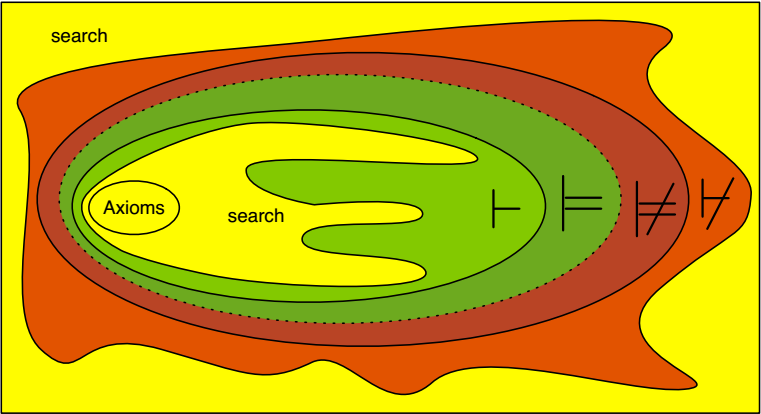
\includegraphics[width=0.65\linewidth]{decidability.png}
    \caption{Illustration of the problem of decidability}
\end{figure}

%%%%%%%%%%%%%%%%%%%%%%%%%%%%%%%%%%%%%%%%%%%%%%%%%%%%%%%%%%%%%%%%%%%%%%%%%%%%%%%%
%%%%%%%%%%%%%%%%%%%%%%%%%%%%%%%%%%%%%%%%%%%%%%%%%%%%%%%%%%%%%%%%%%%%%%%%%%%%%%%%
% CHAPTER : Program proofs
%%%%%%%%%%%%%%%%%%%%%%%%%%%%%%%%%%%%%%%%%%%%%%%%%%%%%%%%%%%%%%%%%%%%%%%%%%%%%%%%
%%%%%%%%%%%%%%%%%%%%%%%%%%%%%%%%%%%%%%%%%%%%%%%%%%%%%%%%%%%%%%%%%%%%%%%%%%%%%%%%

  \chapter{Program Proofs}
  \label{chap:Program Proofs}

%%%%%%%%%%%%%%%%%%%%%%%%%%%%%%%%%%%%%%%%%%%%%%%%%%%%%%%%%%%%%%%%%%%%%%%%%%%%%%%%
% SECTION : Sequential programs
%%%%%%%%%%%%%%%%%%%%%%%%%%%%%%%%%%%%%%%%%%%%%%%%%%%%%%%%%%%%%%%%%%%%%%%%%%%%%%%%
  \section{Sequential Programs}
  \label{sec:Sequential Programs}

As a sequential program, we will use our previous example that computes $a^b$.

\begin{lstlisting}[caption={Function computing $a^b$}, captionpos=below]
{
    x=b;
    y=1;
    while (x>0) do {
        y = y * a;
        x = x - 1;
    }
}
\end{lstlisting}

To be sure that this program does what we think, we need to prove
$$
\{ b \ge 0\} S \{ y = a^b \}
$$

    \subsection{Assignment}

    \subsubsection{Rule}

    $$
    \frac{}
    { \{ p[E/V] \} V = E; \{ p \} }
    $$

    $$
    \frac{}
    { \{ p(E) \} V = E ; \{ p(V) \} }
    $$

    \subsubsection{Example}
    If $p(E)$ holds before $x = E;$ then $p(x)$ holds after.

    \begin{minipage}{0.45\linewidth}
        \begin{tabular}{ll}
            \toprule
            a & 2 \\
            \midrule
            b & 3 \\
            \midrule
            x & ? \\
            \midrule
            y & ? \\
            \bottomrule
        \end{tabular}
        $x = b;$
        \begin{tabular}{ll}
            \toprule
            a & 2 \\
            \midrule
            b & 3 \\
            \midrule
            x & 3 \\
            \midrule
            y & ? \\
            \bottomrule
        \end{tabular}
    \end{minipage}
    \bigskip
    \begin{minipage}{0.45\linewidth}
        \begin{tabular}{ll}
            \toprule
            a & 2 \\
            \midrule
            b & 3 \\
            \midrule
            x & 3 \\
            \midrule
            y & 2 \\
            \bottomrule
        \end{tabular}
        x = x - 1;
        \begin{tabular}{ll}
            \toprule
            a & 2 \\
            \midrule
            b & 3 \\
            \midrule
            x & 2 \\
            \midrule
            y & 2 \\
            \bottomrule
        \end{tabular}
    \end{minipage}

    \subsubsection{Left construction}

    We will use the \textit{left-constructive} approach, such that with the
    last rule, we will start from $p$ to build $p[E/V]$. \newline

    \textbf{Left construction} is a proof strategy for $\{ p \} S \{ q\}$ where
    a precondition $p$ for $S$ is derived mechanically from a postcondition $q$.
    \newline

    An inference rule
    $$
    \frac{\{ {p}_{1} {S}_{1} \{ {q}_{1} \} \ldots \{ {p}_{n} \} {S}_{n} \{ {q}_{n}\}}
    { \{ p \} S \{ q \}}
    $$
    is \textit{left-constructive} iff it allows left construction on the
    conclusion, assuming left construction on the premises, i.e. derive $p$
    from $q$, assuming one can derive each ${p}_{i}$ from $q_{i}$ (in some
    order). Concretely, a \textbf{left-constructive rule} has the form
    $$
    \frac{ \{ {P}_{1} \} {S}_{1} \{ {q}_{1} \} \ldots \{ {P}_{n} \} {S}_{n} \{ {q}_{n} \} }
    { \{ p \} S \{ Q \} }
    $$
    where (for some ordering of the premises)
    \begin{itemize}
        \item $Q, {P}_{1}, \ldots, {P}_{n}$ are simple logic variables
        \item Each ${q}_{i}$ is expressed in termes of $S$ and $Q, {P}_{1}, \ldots, {P}_{i-1}$
        \item $p$ is expressed in termes of $S$ and $Q, {P}_{1}, \ldots, {P}_{n}$
    \end{itemize}

    \subsubsection{Right construction}

    The \textbf{right construction} is also possible but less convenient, the
    inference rule is
    $$
    \frac{}
    { \{ p \} V=E; \{ \exists {V}_{0} \cdot p[{V}_{0}/V] \land V = E[{V}_{0}/V] \} }
    $$
    where ${V}_{0}$ is the old value of $V$ which is lost in the assignment.
    This is more complex because it introduces $\exists$ quantifiers.

    \subsection{Consequence}

    \subsubsection{Rule}

    The following rule is the heart of mechanical proofs (WP calculus,
    verification conditions):

    $$
    \frac{ p \Rightarrow p' , \{ p' \} S \{ q' \} , q' \Rightarrow q }
    { \{ p \} S \{ q \} }
    $$

    This is a purely logical rule, independent from the programming language.
    $p \Rightarrow p'$, $q' \Rightarrow q$ are assertions, which connect Hoare
    logic with the underlying assertion logic (assertions to be proven in an
    auxiliary proof system). The underlying meaning of this rule is that
     $\{ p \} S \{ q \}$ remains valid if we strenghten $p$ and/or weaken $q$.

    \subsubsection{Example}

    The left construction has a consequence, for example we can prove for the
    assignment:
    $$
    \{ x \cdot x = {x}^{2} \}\quad y = x * x; \quad \{ y = {x}^{2} \}
    $$

    But what if we want to deduce
    $$
    \{ true \}\quad y = x*x; \quad \{ y = {x}^{2} \}
    $$
    $$
    \{ true \}\quad y = x*x; \quad \{ y \ge 0 \}
    $$

    This is valid since
    $$
    \{ true \} \Rightarrow \{ x \cdot x = {x}^{2} \} S \{ y = {x}^{2} \} \Rightarrow \{ y \ge 0 \}
    $$
    but this is \textit{not derivable} by the assignment rule.

    \subsection{Sequence}

    \subsubsection{Rule}

    $$
    \frac{ \{ {p}_{0} \} {S}_{1} \{ {p}_{1} \}, \ldots, \{ {p}_{n-1} \} {S}_{n} \{ {p}_n \} }
    { \{ {p}_{0} \} \{ {S}_{1} \ldots {S}_{n} \} \{ {p}_{n} \} }
    $$

    In particular,
    $$
    \frac{}
    { \{ p \} \{ \} \{ p \} }
    $$

    The sequence rule is \textbf{left-constructive}, if for each
    $\{ {p}_{i-1}\} {S}_{i} \{ {p}_{i} \}$, we can build ${p}_{i-1}$ from ${p}_{i}$,
    then we can build ${p}_{0}$ from ${p}_{n}$ (via ${p}_{n-1}$ then ${p}_{n-2}$,
    etc.). If some ${S}_{i}$ is not left-constructive, we must \enquote{guess}
    ${p}_{i-1}$. The sequence rule is also right-constructive but this will be
    less useful.

    \subsubsection{Example}

    The principle is to introduce \textit{intermediate conditions}:
    \bigskip

    \begin{minipage}{\linewidth}
        \begin{minipage}{0.4\linewidth}
            $$ \{ y \cdot a = {a}^{b-(x-1)} \}$$
            $$ y = y * a; $$
            $$ \{ y = {a}^{b-(x-1)} \} $$
            \bigskip
            $$ \{ y = {a}^{b-(x-1)} \} $$
            $$ x = x - 1; $$
            $$ \{ y = {a}^{b-x} \} $$
        \end{minipage}
        \begin{minipage}{0.05\linewidth}
            \Huge $$ \vdash $$
        \end{minipage}
        \begin{minipage}{0.4\linewidth}
            $$ \{ y \cdot a = {a}^{b-(x-1)} \} $$
            $$ \{ y = y * a; \} $$
            $$ x = x - 1; $$
            $$ \{ y = {a}^{b-x} \} $$
        \end{minipage}
    \end{minipage}

    \subsection{Choice}

    \subsubsection{Rule}

    We can define a \textbf{top-down} inference rule, from $p$ and $q$
    (conclusion) we can build $p \land B$, $p \land \lnot B$ (premisses)

    $$
    \frac
    { \{ p \land B \} S_1 \{ q \}, \{ p \land \lnot B \} S_2 \{ q \} }
    { \{ p \} \textrm{ if } (B) \textrm{ then } S_1 \textrm{ else } S_2 \{ q \} }
    $$

    There exists a \textbf{left-constructive} variant

    $$
    \frac
    { \{ p_1 \} S_1 \{ q \}, \{ p_2 \} S_2 \{ q \} }
    { \{ (B \land p_1 ) \lor (\lnot B \land p_2 ) \} \textrm{ if } (B) \textrm{ then } S_1 \textrm{ else } S_2 \{ q \} \} }
    $$

    \subsection{Loop}

    We want to prove

    \begin{center}
    $$\{ x \ge 0 \land x = b \land y =1 \}$$
    \begin{minipage}{0.3\linewidth}
\begin{lstlisting}
while (x > 0) do {
    y = y * a;
    x = x -1;
}
\end{lstlisting}
    \end{minipage}
    $$y = {a}^{b}$$
    \end{center}

    To prove it, we use a \textbf{loop invariant} $y = {a}^{b-x} \land x \ge 0$
    and we denote it $I(x,y)$ for short. We \textit{prove} that the invariant
    is \textbf{preserved by the body} of the loop and we \textit{infer} that
    the invariant is \textbf{preserved by the loop}.

    \subsubsection{Preserved invariant}

    Let $I(x,y) \equiv y = {a}^{b-x} \land x \ge 0$ \newline

    We have:

    \begin{eqnarray*}
        I(x,y) \land x > 0 \Rightarrow I(x-1, y \cdot a) & \textrm{(assertion)} \\
        \{ I(x-1, y \cdot a) \} y = y * a; \{ I(x-1, y) \} & \textrm{(assignment)} \\
        \{ I(x-1, y) \} x = x - 1; \{ I(x,y) & \textrm{(assigment)}
    \end{eqnarray*}

    Hence we infer (sequence, consequence):
    $$
    \{ I(x,y) \land x > 0 \} \{ y = y*a; x=x-1; \} \{ I(x,y) \}
    $$

    \subsubsection{Derivation}

    Let $I(x,y) \equiv y = {a}^{b-x} \land x \ge 0$, we have

    $$
    \{ I(x,y) \land x > 0 \} \{ y=y*a; x=x-1; \} \{ I(x,y) \}
    $$

    \bigskip
    We can infer (loop):

    \begin{minipage}{\linewidth}
        \begin{minipage}[c]{0.3\linewidth}
            $$\{ I(x,y) \}$$
        \end{minipage}
        \begin{minipage}[c]{0.3\linewidth}
            \centering
\begin{lstlisting}
while (x > 0) do {
    y = y * a;
    x = x-1;
}
\end{lstlisting}
        \end{minipage}
        \begin{minipage}[c]{0.3\linewidth}
            $$\{ I(x,y) \land x \le 0 \}$$
        \end{minipage}
    \end{minipage}

    \subsubsection{Consequence}

    Let $I(x,y) \equiv y = {a}^{b-x} \land x \ge 0$, we have
    \bigskip

    \begin{minipage}{\linewidth}
        \begin{minipage}{0.3\linewidth}
            $$\{ I(x,y) \}$$
        \end{minipage}
        \begin{minipage}[c]{0.3\linewidth}
            \centering
\begin{lstlisting}
while (x > 0) do {
    y = y * a;
    x = x-1;
}
\end{lstlisting}
        \end{minipage}
        \begin{minipage}[c]{0.3\linewidth}
            $$\{ I(x,y) \land x \le 0 \}$$
        \end{minipage}
    \end{minipage}

    and also:

    \begin{eqnarray*}
        (x \ge 0 \land x = b \land y = 1) \Rightarrow I(x,y) & \textrm{(assertion)} \\
        (I(x,y) \land x \le 0) \Rightarrow (y = {a}^{b}) & \textrm{(assertion)}
    \end{eqnarray*}

    Hence (consequence):

    \begin{minipage}[c]{\linewidth}
        \begin{minipage}[c]{0.3\linewidth}
            $$\{ x \ge 0 \land x = b \land y = 1 \}$$
        \end{minipage}
        \begin{minipage}[c]{0.3\linewidth}
            \centering
\begin{lstlisting}
while (x>0) do {
    y = y*a;
    x = x-1;
}
\end{lstlisting}
        \end{minipage}
        \begin{minipage}[c]{0.3\linewidth}
            $$\{ y = {a}^{b} \}$$
        \end{minipage}
    \end{minipage}

    Q.E.D.

    \subsubsection{Rule}

    $I$ is the invariant, this rule is \textbf{non-constructive} (i.e.\ not
    top-down, not left-constructive).

    \subsection{Choosing the invariant}

    $$
    \frac
    { \{ I \land B \} S \{ I \} }
    { \{ I \} \textrm{ while } (B) \textrm{ do } S \{ I \land \lnot B \} }
    $$

    The invariant $I$ must be \enquote{guessed}, it does not derive mechanically
    from the property to be proven. $p$ is in general too strong to be the
    invariant and $q$ is too weak, we need an intermediate $I$ such that
    $p \Rightarrow I$ and $I \land \lnot B \Rightarrow q$.

    \subsubsection{Example: Conclusion}

    We wanted to prove:

    $$
    \{ b \ge 0 \}
    $$
    $$
    \{ x =b ; y=1; \textrm{ while } (x>0) \textrm{ do } \{ \ldots \} \}
    $$
    $$
    \{ y = {a}^{b} \}
    $$

    \begin{eqnarray*}
        (b \ge 0) \Rightarrow (b \ge 0 \land b =b \land 1 = 1) & \textrm{(assertion)} \\
        \{ b \ge 0 \land b = b \land 1 = 1 \} \{ x=b; y=1; \} \{ x \ge 0 \land x = b \land y = 1 \} & \textrm{(assignment, sequence)} \\
        \{ X \ge 0 \land x =b \land y = 1 \} \textrm{ while } (x>0) \textrm{ do } \{ \ldots \} \{ y = {a}^{b} \} & \textrm{(loop, consequence)}
    \end{eqnarray*}

    Hence the property (sequence, consequence)

    \subsection{Total correctness}

    \subsubsection{Rule}

    For this rule, we do not need to change the rules already defined for
    consequence, assignment, sequence and choice. Here is the one for the
    loop:

    \begin{center}
    \begin{minipage}{0.6\linewidth}
    \begin{framed}
    \[
    \inference{
        {\begin{array}{c}
            \lbrack I \land B \rbrack S [I], \\
            \lbrack I \land B \land E = z \rbrack S [E < z], \\
            I \Rightarrow E \ge 0
        \end{array}}
    }
    {[I] \textrm{ while } (B) \textrm{ do } S [I \land\lnot B]}
    \]
    \end{framed}
    \end{minipage}
    \end{center}

    $E$ is an integer-type expression, if we allow real expression we have the
    risk that it could decrease indefinitely (for example, x=1 and a loop until
    $x == 0$ where $x:=x/2$ would make $x$ decreases but never reach 0). $z$
    must be a fresh variable (that does not occur in $S$, $B$, $E$, $I$). This
    rule is \textbf{non-constructive} as we must \enquote{guess} $E$ and $I$.

    \subsubsection{Example}

    We want to prove:
    \begin{center}
    $$[b \ge 0]$$
    \begin{minipage}{0.4\linewidth}
\begin{lstlisting}
{
    x = b;
    y = 1;
    while (x > 0) do ...
}
\end{lstlisting}
    \end{minipage}
    $$[y = a^{b}]$$
    \end{center}

    \bigskip

    Remember that $\{ p \} S \{ q \}$ is the proof of partial correctness and
    here we talk about $[p] S [q]$ which adds \textbf{termination}. The only
    thing that can prevent the termination is the loop, the termination of the
    loop will lead to the termination of the program:

    \begin{center}
    $$[ x \ge 0 \land x =b \land y=1]$$
    \begin{minipage}{0.3\linewidth}
\begin{lstlisting}
while (x>0) do {
    y = y*a;
    x = x -1;
}
\end{lstlisting}
    \end{minipage}
    $$y = {a}^{b}$$
    \end{center}

    \bigskip

    We want to prove
    \begin{center}
    $$[x \ge 0 \land x =b \land y =1]$$
    \begin{minipage}{0.3\linewidth}
\begin{lstlisting}
while (x>0) do {
    y = y * a;
    x = x -1;
}
\end{lstlisting}
    \end{minipage}
    $$[y = {a}^{b}]$$
    \end{center}

    \bigskip

    We add a \textbf{loop variant} $x$ to the variant $y = {a}^{b-x} \land x \ge 0$
    for partial correctness. We prove that the \textbf{variant decreases} on
    every execution of the body of the loop: \newline

    \begin{center}
    $$[y = {a}^{b-x} \land x \ge 0 \land x > 0 \land x = {x}_{0}]$$
    \begin{minipage}{0.5\linewidth}
\begin{lstlisting}
{ y = y * a; x = x-1; }
\end{lstlisting}
    \end{minipage}
    $$[x < {x}_{0}]$$
    \end{center}

    \bigskip

    We prove that the variant \textbf{remains positive or null} within the
    scope of the invariant:

    $$
    y = {a}^{b-x} \land x \ge 0 \Rightarrow x \ge 0
    $$

    As you can see, this is an assertion.

    We can deduce the desired property as for partial correctness:

    \begin{center}
    $$[y = {a}^{b-x} \land x \ge 0]$$
    \begin{minipage}{0.3\linewidth}
\begin{lstlisting}
while (x > 0) do {
    y = y * a;
    x = x - 1;
}
\end{lstlisting}
    \end{minipage}
    $$[y = {a}^{b-x} \land x \ge 0 \land 0 \land x \le 0]$$
    \end{center}

    \subsubsection{Well-founded termination}

    As working only with integer isn't always enough, we can generalize the
    termination for non-integer variants if there exists a well-founded order
    on the variable discussed in the variant. We write the rule as

    \begin{center}
    \begin{minipage}{0.6\linewidth}
    \begin{framed}
    \[
        \inference{
            {\begin{array}{c}
                \lbrack I \land B \rbrack\quad S\quad [I], \\
                \lbrack I \land B \land E = z \rbrack\quad S\quad [E \prec z], \\
                I \Rightarrow W(E)
            \end{array}}
        }
        {
        \lbrack I\rbrack\quad \textrm{ while } (B) \textrm{ do } S\quad [I \land\lnot{} B]
        }
    \]
    \end{framed}
    \end{minipage}
    \end{center}

    where
    \begin{itemize}
        \item $E$ is an expression of type $T$ (domain ${D}_{T}$)
        \item $\prec$ is a binary predicate (relation) over ${D}_{T} \times {D}_{T}$
        \item $W$ is a predicate defining a subset of $D_T$
        \item $[[\prec]]$ is \textbf{well-founded order} over $[[W]] \subseteq {D}_T$
        \item $z$ is a fresh variable (not occuring in $S$, $B$, $E$, $I$)
    \end{itemize}

    \subsection{Constance}

    If the execution of $S$ doesn't affect any variable in $p$, i.e.
    if $vars(p) \cap assign(S) = \oslash$ then

    \begin{center}
    \begin{minipage}{0.5\linewidth}
    \begin{framed}
        \[
        \inference{}
        { \{ p \} S \{ p \}}
    \]
    \end{framed}
    \end{minipage}
    \end{center}

    \subsection{Conjunction}

    \begin{center}
    \begin{minipage}{0.5\linewidth}
    \begin{framed}
        \[
        \inference{ \{ p \} S \{ q \}, \{ p' \} S \{ q' \} }
        { \{ p \land p' \} S \{ q \land q' \} }
        \]
    \end{framed}
    \end{minipage}
    \end{center}

    \subsection{Disjunction}

    \begin{center}
    \begin{minipage}{0.5\linewidth}
    \begin{framed}
        \[
        \inference{ \{ p \} S \{ q \}, \{ p' \} S \{ q' \} }
        { \{ p \lor p' \} S \{ q \lor q' \} }
        \]
    \end{framed}
    \end{minipage}
    \end{center}

    % TODO : We could add the full proof for power

    \subsection{On soundness and completeness}

    The five proof rules (consequence, assignment, sequence, choice, loop)
    generate a set of theorems $\Phi$ (and a total correctness variant
    $\Phi_{\perp}$).

    \begin{eqnarray*}
        \vdash \{ p \} S \{ q \} & \textrm{iff} & \{ p \} S \{ q \} \in \Phi \\
        \vdash [ p ] S [ q ] & \textrm{iff} & [ p ] S [ q ] \in \Phi_{\perp}
    \end{eqnarray*}

    As a reminder, \textit{soundness} corresponds to \enquote{if
    $\vdash \{ p \} S \{ q \}$ then $\models \{ p \} S \{ q \}$}.
    \textit{Completeness} correspond to \enquote{if $\models \{ p \} S \{ q \}$
    then $\vdash \{ p \} S \{ q \}$}.

    \subsubsection{Soundness: application on assignment}

    Remember the rule for assignment:

    \begin{center}
        \begin{minipage}{0.4\linewidth}
        \begin{framed}
            \inference{}
            { \{ p[E/V] \} V = E; \{ p \} }
        \end{framed}
        \end{minipage}
    \end{center}

    Let $\sigma \models p[E/V]$

    \begin{description}
        \item[Semantics] $(V = E; , \sigma) \longrightarrow (\{\}, \sigma[V := \sigma(E)]) $
        \item[Substitution lemma] $\sigma \models p[E/V]$ iff $\sigma[V:=\sigma(E)] \models p$
    \end{description}


%%%%%%%%%%%%%%%%%%%%%%%%%%%%%%%%%%%%%%%%%%%%%%%%%%%%%%%%%%%%%%%%%%%%%%%%%%%%%%%%
% SECTION : Verification conditions
%%%%%%%%%%%%%%%%%%%%%%%%%%%%%%%%%%%%%%%%%%%%%%%%%%%%%%%%%%%%%%%%%%%%%%%%%%%%%%%%
  \section{Verification Conditions}
  \label{sec:Verification Conditions}
%%%%%%%%%%%%%%%%%%%%%%%%%%%%%%%%%%%%%%%%%%%%%%%%%%%%%%%%%%%%%%%%%%%%%%%%%%%%%%%%
% SECTION : Procedures
%%%%%%%%%%%%%%%%%%%%%%%%%%%%%%%%%%%%%%%%%%%%%%%%%%%%%%%%%%%%%%%%%%%%%%%%%%%%%%%%
  \section{Procedures}
  \label{sec:Procedures}

%%%%%%%%%%%%%%%%%%%%%%%%%%%%%%%%%%%%%%%%%%%%%%%%%%%%%%%%%%%%%%%%%%%%%%%%%%%%%%%%
% SECTION : Recursion
%%%%%%%%%%%%%%%%%%%%%%%%%%%%%%%%%%%%%%%%%%%%%%%%%%%%%%%%%%%%%%%%%%%%%%%%%%%%%%%%
  \section{Recursion}
  \label{sec:Recursion}

%%%%%%%%%%%%%%%%%%%%%%%%%%%%%%%%%%%%%%%%%%%%%%%%%%%%%%%%%%%%%%%%%%%%%%%%%%%%%%%%
% SECTION : Data Structures
%%%%%%%%%%%%%%%%%%%%%%%%%%%%%%%%%%%%%%%%%%%%%%%%%%%%%%%%%%%%%%%%%%%%%%%%%%%%%%%%
  \section{Data Structures}
  \label{sec:Data Structures}

  \section{Data abstraction}
  \label{sec:Data abstraction}


%%%%%%%%%%%%%%%%%%%%%%%%%%%%%%%%%%%%%%%%%%%%%%%%%%%%%%%%%%%%%%%%%%%%%%%%%%%%%%%%
% SECTION : Reactive Programs
%%%%%%%%%%%%%%%%%%%%%%%%%%%%%%%%%%%%%%%%%%%%%%%%%%%%%%%%%%%%%%%%%%%%%%%%%%%%%%%%
  \section{Reactive Programs}
  \label{sec:Reactive Programs}
  \subsection{From application to reactive}
  \label{sub:From application to reactive}
  \subsubsection{Applicative programs}
  \label{subs:Applicative programs}
  \subsubsection{Reactive programs}
  \label{subs:Reactive programs}
  \subsubsection{Prooofs of reactive programs}
  \label{subs:Prooofs of reactive programs}
  \subsection{Non-deterministic programs}
  \label{sub:Non-deterministic programs}
  \subsubsection{Guarded commands}
  \label{subs:Guarded commands}
  \subsubsection{Deadlock}
  \label{subs:Deadlock}
  \subsubsection{Strong vs. weak total correctness}
  \label{subs:Strong vs. weak total correctness}
  \subsection{Concurrent programs}
  \label{sub:Concurrent programs}
  \subsubsection{Interleaving}
  \label{subs:Interleaving}
  \subsubsection{Atomicity}
  \label{subs:Atomicity}
  \subsubsection{Disjoint parallel programs}
  \label{subs:Disjoint parallel programs}
  \subsubsection{Compositional proofs}
  \label{subs:Compositional proofs}
  \subsubsection{General concurrent programs}
  \label{subs:General concurrent programs}
  \subsubsection{Interference-free proofs}
  \label{subs:Interference-free proofs}
  \subsubsection{Fairness}
  \label{subs:Fairness}


%%%%%%%%%%%%%%%%%%%%%%%%%%%%%%%%%%%%%%%%%%%%%%%%%%%%%%%%%%%%%%%%%%%%%%%%%%%%%%%%
%%%%%%%%%%%%%%%%%%%%%%%%%%%%%%%%%%%%%%%%%%%%%%%%%%%%%%%%%%%%%%%%%%%%%%%%%%%%%%%%
% CHAPTER : Program validation
%%%%%%%%%%%%%%%%%%%%%%%%%%%%%%%%%%%%%%%%%%%%%%%%%%%%%%%%%%%%%%%%%%%%%%%%%%%%%%%%
%%%%%%%%%%%%%%%%%%%%%%%%%%%%%%%%%%%%%%%%%%%%%%%%%%%%%%%%%%%%%%%%%%%%%%%%%%%%%%%%

  \chapter{Program Validation}
  \label{chap:Program Validation}

%%%%%%%%%%%%%%%%%%%%%%%%%%%%%%%%%%%%%%%%%%%%%%%%%%%%%%%%%%%%%%%%%%%%%%%%%%%%%%%%
% SECTION : State-Based Models
%%%%%%%%%%%%%%%%%%%%%%%%%%%%%%%%%%%%%%%%%%%%%%%%%%%%%%%%%%%%%%%%%%%%%%%%%%%%%%%%
  \section{State-Based Models}
  \label{sec:State-Based Models}
  \subsection{Introduction}
  \label{sub:Introduction}
  \subsection{Summary}
  \label{sub:Summary}
  \subsection{Models of Reactive Programs?}
  \label{sub:Models of Reactive Programs?}
  \subsection{State machines}
  \label{sub:State machines}
  \subsubsection{Principles}
  \label{subs:Principles}
  \subsubsection{Definition}
  \label{subs:Definition}
  \subsubsection{Example}
  \label{subs:Example}
  \subsubsection{Traces}
  \label{subs:Traces}
  \subsection{Infinite executions}
  \label{sub:Infinite executions}
  \subsubsection{Example of State Machine}
  \label{subs:Example of State Machine}
  \subsection{State machines and programs}
  \label{sub:State machines and programs}
  \subsubsection{Example of Program}
  \label{subs:Example of Program}
  \subsubsection{Interpreted State Machines}
  \label{subs:Interpreted State Machines}
  \subsection{Kripke structure}
  \label{sub:Kripke structure}
  \subsubsection{Example}
  \label{subs:Example}
  \subsubsection{Interpretation on Programs}
  \label{subs:Interpretation on Programs}
  \subsection{Program Locations}
  \label{sub:Program Locations}
  \subsection{Temporal logic}
  \label{sub:Temporal logic}
  \subsection{LTL}
  \label{sub:LTL}
  \subsubsection{Principle}
  \label{subs:Principle}
  \subsubsection{Syntax}
  \label{subs:Syntax}
  \subsubsection{Semantics over traces}
  \label{subs:Semantics over traces}
  \subsubsection{Semantics over structures}
  \label{subs:Semantics over structures}
  \subsubsection{Examples (safety)}
  \label{subs:Examples (safety)}
  \subsubsection{Examples (liveness)}
  \label{subs:Examples (liveness)}
  \subsubsection{Examples (deadlock)}
  \label{subs:Examples (deadlock)}
  \subsubsection{Until vs Unless}
  \label{subs:Until vs Unless}
  \subsubsection{Quid of Hoare Logic?}
  \label{subs:Quid of Hoare Logic?}
  \subsubsection{Examples (pre/post)}
  \label{subs:Examples (pre/post)}
  \subsection{Other temporal logics}
  \label{sub:Other temporal logics}
  \subsection{Summary}
  \label{sub:Summary}






%%%%%%%%%%%%%%%%%%%%%%%%%%%%%%%%%%%%%%%%%%%%%%%%%%%%%%%%%%%
%% SECTION : MODEL CHECKING
%%%%%%%%%%%%%%%%%%%%%%%%%%%%%%%%%%%%%%%%%%%%%%%%%%%%%%%%%%%
  \section{Model Checking}
  \label{sec:Model Checking}
  \subsection{Recall}
  \label{sub:Recall}
  \subsubsection{State Machines}
  \label{subs:State Machines}
  \subsubsection{Temporal logic}
  \label{subs:Temporal logic}
  \subsubsection{Summary}
  \label{subs:Summary}
  \subsection{Definition}
  \label{sub:Definition}
  \subsection{Basic principles}
  \label{sub:Basic principles}
  \subsection{Verification vs. Refutation}
  \label{sub:Verification vs. Refutation}
  \subsection{Automata}
  \label{sub:Automata}
  \subsection{Two versions of model-checking}
  \label{sub:Two versions of model-checking}
  \subsection{Reachability}
  \label{sub:Reachability}
  \subsection{LTL property}
  \label{sub:LTL property}
  \subsection{Infinite traces}
  \label{sub:Infinite traces}
  \subsection{Büchi Automata}
  \label{sub:Büchi Automata}
  \subsubsection{From LTL to Büchi}
  \label{subs:From LTL to Büchi}
  \subsubsection{Examples}
  \label{subs:Examples}
  \subsection{Product Automaton}
  \label{sub:Product Automaton}
  \subsection{Repeated reachability}
  \label{sub:Repeated reachability}
  \subsubsection{Remarks}
  \label{subs:Remarks}
  \subsubsection{Example}
  \label{subs:Example}
  \subsubsection{Properties}
  \label{subs:Properties}
  \subsection{Model-checking without LTL?}
  \label{sub:Model-checking without LTL?}
  \subsection{Complexity}
  \label{sub:Complexity}
  \subsubsection{State space explosion}
  \label{subs:State space explosion}
  \subsection{Partial-order reduction}
  \label{sub:Partial-order reduction}
  \subsection{Spin}
  \label{sub:Spin}
  \subsubsection{Promela}
  \label{subs:Promela}
  \subsubsection{Execution}
  \label{subs:Execution}
  \subsection{Symbolic Model Checking}
  \label{sub:Symbolic Model Checking}
  \subsection{Binary Decision Diagrams (BDD)}
  \label{sub:Binary Decision Diagrams (BDD)}
  \subsubsection{Definition}
  \label{subs:Definition}
  \subsubsection{Example}
  \label{subs:Example}
  \subsubsection{Ordering of variables}
  \label{subs:Ordering of variables}
  \subsection{SAT solving}
  \label{sub:SAT solving}
  \subsection{Bounded model-checking}
  \label{sub:Bounded model-checking}
  \subsubsection{Discussion}
  \label{subs:Discussion}
  \subsection{Model Checking for Programs}
  \label{sub:Model Checking for Programs}
  \subsubsection{Traditional model checkers}
  \label{subs:Traditional model checkers}
  \subsubsection{Java PathFinder}
  \label{subs:Java PathFinder}
  \subsection{Test vs. Model checking}
  \label{sub:Test vs. Model checking}
  \subsection{Partial Model-Checking}
  \label{sub:Partial Model-Checking}
  \subsection{Exploration strategies}
  \label{sub:Exploration strategies}
  \subsection{State Hashing}
  \label{sub:State Hashing}
  \subsection{Stateless Model-Checking}
  \label{sub:Stateless Model-Checking}
  \subsubsection{Verisoft}
  \label{subs:Verisoft}
  \subsection{Runtime Monitoring}
  \label{sub:Runtime Monitoring}
  \subsection{Summary}
  \label{sub:Summary}

\end{document}
